\documentclass[11pt]{beamer}
\usetheme{Madrid}
\usepackage[utf8]{inputenc}
\usepackage{amsmath}
\usepackage{amsfonts}
\usepackage{amssymb}
\usepackage{graphicx}
\usepackage{mathptmx}
\usepackage{chancery}
%\author{}
%\title{}
%\setbeamercovered{transparent} 
%\setbeamertemplate{navigation symbols}{} 
%\logo{} 
%\institute{} 
%\date{} 
%\subject{} 
\begin{document}

\begin{frame}

\begin{figure}[center]
  
\includegraphics[width=3.5cm, height=4cm]{Img/ULA.png}
\end{figure}


{\bf \large Nombre  :} \large HUALLPAR DORADO, Jhoel \\
{\bf \large Curso   :} \large Estructura de Datos \\
{\bf \large Docente :} \large Luciano Arnaldo Romero Calla \\
{\bf \large Tema    :} \Large Fibonacci Heap\\
{\bf \large Correo  :} \large jhuallpard@ulasalle.edu.pe\\

\titlepage
\end{frame}

\begin{frame} {\bf \large \rightline{Fibonacci Heap   *}}
\tableofcontents
{\center \bf \Huge \color{purple} \texttt{FIBONACCI HEAP} \\}

\begin{figure}[center]
  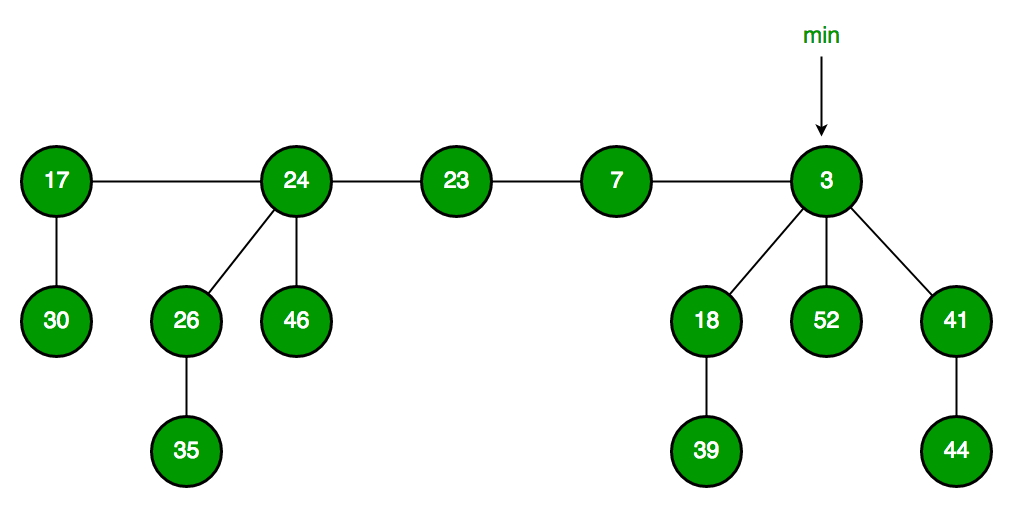
\includegraphics[width=10cm, height=5cm]{Img/FH.png}
\end{figure}

\end{frame}

\begin{frame} {\bf \large \rightline{Fibonacci Heap   *}}
\tableofcontents
{\center \bf \Large CONTENIDO \\}

\begin{figure}[right]
  
\includegraphics[width=3.5cm, height=4cm]{Img/Indice.jpg}
\end{figure}

\begin{enumerate}
\item Introducci\'on
\item Insert
\item Delete
\item Delete
\item Delete
\item Delete
\end{enumerate}

\end{frame}

\begin{frame}{\bf \large \rightline{Fibonacci Heap   *}}

{\center \bf \large INTRODUCCI\'ON \\}

\end{frame}

\begin{frame}{\bf \large \rightline{Fibonacci Heap   *}}

{\center \bf \large INSERT \\}

\end{frame}


\end{document}